\documentclass{article}
\usepackage{fourier}
\usepackage[margin=0.498in]{geometry}
\usepackage{graphicx}
% Redefine \includegraphics so that, unless explicit options are
% given, the image width will not exceed the width of the page.
% Images get their normal width if they fit onto the page, but
% are scaled down if they would overflow the margins.
\makeatletter
\def\ScaleIfNeeded{%
  \ifdim\Gin@nat@width>\linewidth
    \linewidth
  \else
    \Gin@nat@width
  \fi
}
\makeatother
\let\Oldincludegraphics\includegraphics
{%
 \catcode`\@=11\relax%
 \gdef\includegraphics{\@ifnextchar[{\Oldincludegraphics}{\Oldincludegraphics[width=\ScaleIfNeeded]}}%
}%

\title{\textbf{CS4110 -- Assignment 2\\Cache Simulator}}
\author{Viswajith V -- CS11B028\\Sriram V -- CS11B058}
\date{September 12, 2014}

\begin{document}

\maketitle

\section{Architecture}
The architecture assumed while modelling the simulator was that of a strictly inclusive, write-back, n-way set associative multilevel cache. The associativity and number of levels are provided by means of a config file, and write-back of a block is performed only when it needs to be evicted. If a block is to be evicted at a level $i$, we also invalidate this block (should it exist) at levels $i-1$ to $0$, to ensure inclusivity.\\
Further, this invalidation is done till:
\begin{itemize}
    \item
        The bottom-most level, $L1$ is reached, or
    \item
        A level where the block under consideration has its dirty bit set to $1$. (As part of our eviction algorithm, we maintain an invariant -- a level having a block with its dirty bit set to $1$ is the lowest level that contains this block.)
\end{itemize}
We also assume that if a write miss ends up going all the way up to the main memory, the dirty bit is not set for any of the levels since the data has been written to the main memory. This gets rid of a redundant write that might occur when this block might be evicted in the future.\\
Thus, with this assumed architecture, the number of hits, misses and accesses is exactly equal to the values mentioned on the course forum.\\
The number of extraneous factors in the matrix multiplication code is kept to a minimum by not printing out the result of the matrix. Static initialization was attempted to further reduce their influence, but failed because of the difficulty in assigning contiguous arrays of size $1024 \times 1024$. Hence, we had to go with dynamic initialization.

\section{Observations}

\begin{enumerate}
\item \textbf{ LRU }:\\

\begin{tabular}{ |c|c|c|c|c|c|c|c|c| }
\hline
& \multicolumn{2}{|c|}{Miss Ratio} & \multicolumn{2}{|c|}{Cache Hits} & \multicolumn{2}{|c|}{Memory Accesses} & \multicolumn{2}{|c|}{Latencies} \\  \hline
Dimension & L1 & L2 & L1 & L2 & L1 & L2 & L1 & L2 \\  \hline
8  &  0.011485 & 0.910201 &  1706115 & 1780 &  1746748 & 40209 &  6986992 & 643344 \\ \hline
16  &  0.009718 & 0.909704 &  2025764 & 1795 &  2066464 & 40341 &  8265856 & 645456 \\ \hline
32  &  0.004626 & 0.908227 &  4348818 & 1855 &  4390171 & 41077 &  17560684 & 657232 \\ \hline
64  &  0.002057 & 0.434727 &  22076193 & 25725 &  22168266 & 69295 &  88673064 & 1108720 \\ \hline
128  &  0.001901 & 0.604651 &  160659896 & 120971 &  161280529 & 499612 &  645122116 & 7993792 \\ \hline
256  &  0.001824 & 0.999058 &  1257096073 & 2165 &  1261811277 & 4617959 &  752277812 & 73887344 \\ \hline
512  &  0.015441 & 0.852979 &  1386493075 & 3196999 &  1431490884 & 40385223 &  1430996240 & 646163568 \\ \hline
1024  &  0.757688 & 0.096005 &  974387659 & 1293982223 &  455588948 & 1569155801 &  1822355792 & 663310960 \\ \hline
\end{tabular}\\

For the Main Memory:\\

\begin{tabular}{ |c|c|c| }
\hline
Dimension & Memory Accesses & Latencies \\  \hline
8 & 20399 & 4079800 \\ \hline
16 & 20409 & 4081800 \\ \hline
32 & 20680 & 4136000 \\ \hline
64 & 22459 & 4491800 \\ \hline
128 & 194138 & 38827600 \\ \hline
256 & 2324614 & 464922800 \\ \hline
512 & 18656078 & 563751696 \\ \hline
1024 & 137960580 & 1822312224 \\ \hline
\end{tabular}\\\\

\item \textbf{ LFU }:\\

\begin{tabular}{ |c|c|c|c|c|c|c|c|c| }
\hline
& \multicolumn{2}{|c|}{Miss Ratio} & \multicolumn{2}{|c|}{Cache Hits} & \multicolumn{2}{|c|}{Memory Accesses} & \multicolumn{2}{|c|}{Latencies} \\  \hline
Dimension & L1 & L2 & L1 & L2 & L1 & L2 & L1 & L2 \\  \hline
8  &  0.019228 & 0.965106 &  1692751 & 1158 &  1788683 & 65645 &  7154732 & 1050320 \\ \hline
16  &  0.017069 & 0.967093 &  2010726 & 1149 &  2111815 & 69131 &  8447260 & 1106096 \\ \hline
32  &  0.013914 & 0.968450 &  4308239 & 1918 &  4486185 & 120751 &  17944740 & 1932016 \\ \hline
64  &  0.007380 & 0.991798 &  21958449 & 1339 &  22444381 & 325660 &  89777524 & 5210560 \\ \hline
128  &  0.017337 & 0.999449 &  158175146 & 1537 &  166543283 & 5580510 &  666173132 & 89288160 \\ \hline
256  &  0.020727 & 0.999920 &  1233290423 & 2095 &  1311594553 & 52204324 &  951410916 & 835269184 \\ \hline
512  &  0.170019 & 0.999968 &  1168811427 & 7594 &  1887077715 & 478846601 &  1041623732 & 928388976 \\ \hline
1024  &  0.992775 & 0.999996 &  530266406 & 6741 &  1861863476 & 543920866 &  1142480688 & 112799264 \\ \hline
\end{tabular}\\

For the Main Memory:\\

\begin{tabular}{ |c|c|c| }
\hline
Dimension & Memory Accesses & Latencies \\  \hline
8 & 34417 & 6883400 \\ \hline
16 & 35894 & 7178800 \\ \hline
32 & 64022 & 12804400 \\ \hline
64 & 168036 & 33607200 \\ \hline
128 & 2889257 & 577851400 \\ \hline
256 & 26845833 & 1074199304 \\ \hline
512 & 241705891 & 1096537944 \\ \hline
1024 & 1894227516 & 888381152 \\ \hline
\end{tabular}\\\\

\item \textbf{ RR }:\\

\begin{tabular}{ |c|c|c|c|c|c|c|c|c| }
\hline
& \multicolumn{2}{|c|}{Miss Ratio} & \multicolumn{2}{|c|}{Cache Hits} & \multicolumn{2}{|c|}{Memory Accesses} & \multicolumn{2}{|c|}{Latencies} \\  \hline
Dimension & L1 & L2 & L1 & L2 & L1 & L2 & L1 & L2 \\  \hline
8  &  0.012630 & 0.857831 &  1704139 & 3099 &  1755844 & 42404 &  7023376 & 678464 \\ \hline
16  &  0.010660 & 0.862613 &  2023836 & 2996 &  2075550 & 42476 &  8302200 & 679616 \\ \hline
32  &  0.005044 & 0.866146 &  4346992 & 2950 &  4399450 & 43060 &  17597800 & 688960 \\ \hline
64  &  0.001777 & 0.540729 &  22082381 & 18059 &  22170047 & 63556 &  88680188 & 1016896 \\ \hline
128  &  0.001790 & 0.320625 &  160677745 & 195751 &  161298195 & 387192 &  645192780 & 6195072 \\ \hline
256  &  0.002860 & 0.728297 &  1255791873 & 978548 &  1264301235 & 6245414 &  762237644 & 99926624 \\ \hline
512  &  0.024232 & 0.651704 &  1374113350 & 11885590 &  1453465583 & 56485105 &  1518895036 & 903761680 \\ \hline
1024  &  0.481656 & 0.307763 &  1495859617 & 629889241 &  839518377 & 1192488312 &  936893788 & 1899943808 \\ \hline
\end{tabular}\\

For the Main Memory:\\

\begin{tabular}{ |c|c|c| }
\hline
Dimension & Memory Accesses & Latencies \\  \hline
8 & 21092 & 4218400 \\ \hline
16 & 21219 & 4243800 \\ \hline
32 & 21613 & 4322600 \\ \hline
64 & 24749 & 4949800 \\ \hline
128 & 101691 & 20338200 \\ \hline
256 & 2653111 & 530622200 \\ \hline
512 & 22361947 & 177422104 \\ \hline
1024 & 280777090 & 320843152 \\ \hline
\end{tabular}\\\\
\end{enumerate}

\section{Inferences and Explanations for Trends Observed}
\begin{itemize}
    \item
        \begin{figure}[htbp]
        \centering
        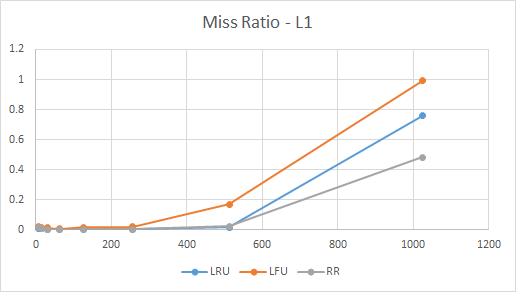
\includegraphics[scale=1.0]{missratio_l1.png}
        \caption{Miss Ratio of L1 (for LRU, LFU and RR) vs Matrix Dimension}
        \end{figure}

        \begin{figure}[htbp]
        \centering
        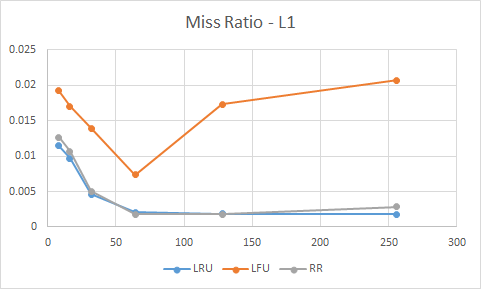
\includegraphics[scale=1.0]{missratio_l1_magnified.png}
        \caption{Miss Ratio of L1 (for LRU, LFU and RR) vs Matrix Dimension (till 256 only)}
        \end{figure}

        \begin{figure}[htbp]
        \centering
        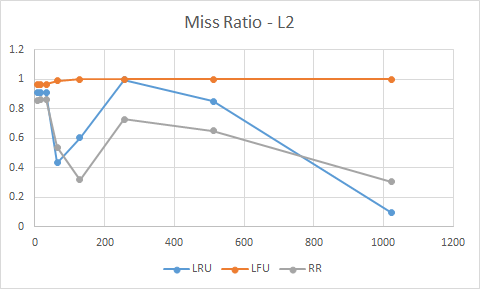
\includegraphics[scale=1.0]{missratio_l2.png}
        \caption{Miss Ratio of L2 (for LRU, LFU and RR) vs Matrix Dimension}
        \end{figure}

        A primary inference we could make from the observed trends is that a heuristic that might seem logical at the surface level, may fail to perform better than a randomized heuristic, if enough thought is not put into its design. We see that LFU performs worse than RR here, and this is because of the temporal and spatial locality of reference. When a new block has been fetched into the cache, it is highly likely that it will be accessed again within a particular time window. However, as it has been freshly fetched, its frequency is still low and hence it has a high chance of being evicted even though it might be required again in the immediate future. Thus, this leads to a thrashing-like behaviour, with a set of blocks being evicted and fetched over and over again, leading to a higher miss ratio that RR (Figures $1$, $2$ and $3$).
    \item
        \begin{figure}[htbp]
        \centering
        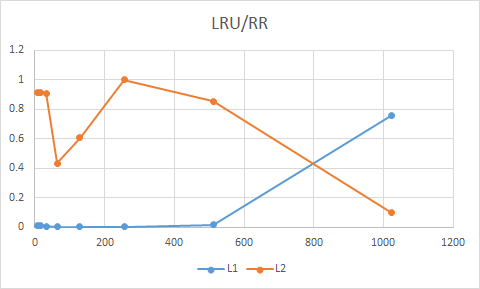
\includegraphics[scale=1.0]{lru_rr.png}
        \caption{Miss Ratios of L1 \& L2 for LRU and RR}
        \end{figure}

        \begin{figure}[htbp]
        \centering
        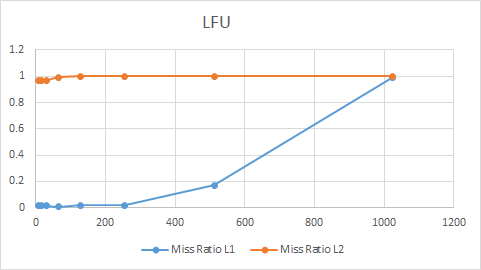
\includegraphics[scale=1.0]{lfu.png}
        \caption{Miss Ratios of L1 \& L2 for LFU}
        \end{figure}

        Yet another observation was the fact that $L1$ always had a very low miss ratio, while it was high for $L2$, except when the dimensions hit $1024$, in which case $L2$ had a lower miss ratio than $L1$ (Figures $4$ and $5$). At lower dimensions, the number of $L1$ cache misses are very few because these misses occur only when data from a different spatial locality is needed, in which case it is has to be fetched (most of the times) from the main memory leading to many $L2$ misses, of these few $L1$ misses.
    \item
        In the case of $1024$ however, due to the fact that $L1$ can store at most $1024$ blocks for the given configuration, and the fact that multiplication would involve fetching a row and a column (thus affecting spatial locality for one of the two, depending on a row-major or column-major based storage), it leads to a large number of misses at $L1$. Thus, these misses are due to space constraints (rather than due to fetches from a different spatial locality \emph{alone}, as in the previous case), which $L2$ handles by providing additional space. This results in an increase in the number of cache hits at $L2$, giving a lower miss ratio than $L1$ in this case.
\end{itemize}

\end{document}
